\hypertarget{a-la-duxe9couverte-des-mystuxe8res-de-rapa-nui}{%
\section{A la découverte des mystères de Rapa
Nui}\label{a-la-duxe9couverte-des-mystuxe8res-de-rapa-nui}}

\emph{Lundi 27 août 2018}

Avant de venir faire un tour sur la "grande Rapa", nous n'avions aucune
idée qu'elle formait le sommet Est du triangle polynésien (dont les
autres sont Hawaï et la Nouvelle Zélande, avec au centre la Polynésie
Française). Même s'il y fait un peu plus frais que sur les îles visitées
durant les dernières semaines, on retrouve des signes de cet héritage un
peu partout. Et en premier lieu, dans les visages que l'on rencontre.
D'autres similarités, dans le désordre : bonjour se dit \emph{Iorana}
(mais accentué à l'espagnole), il y a des chiens errants partout, on
voit des coiffes et des colliers de fleurs, les magasins peuvent être
relativement vides quand le bateau de ravitaillement tarde à arriver,
les palmiers, les églises d'obédiences variées dues aux "guerres de
conversion" du 18ème siècle, les couchers de soleil magnifiques...

\begin{figure}
\centering
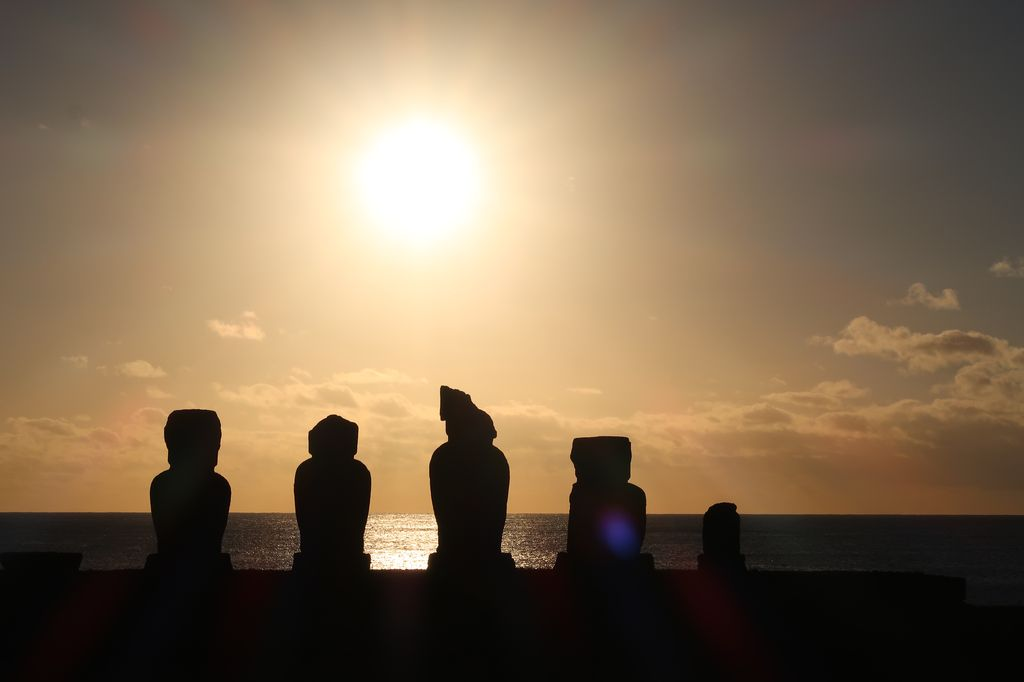
\includegraphics{images/20180827_tahai.JPG}
\caption{Premier et dernier coucher de soleil de notre séjour ont eu
lieu ici, à Tahai.}
\end{figure}

Mais à quels mystères faisons-nous référence dans le titre de ce billet
? Ils sont nombreux \emph{a priori}, sur cette île qui fascine. Qui ont
été les premiers habitants ? Pourquoi et comment ont-ils construit les
colossaux Moais en pierre ? Pourquoi les Moais ont-ils été renversés à
partir du 18ème siècle ? Est-il vrai qu'on y pratiquait l'épreuve de
l'homme-oiseau où il s'agissait de ramener intact le premier œuf d'un
oiseau migrateur après avoir descendu une falaise mortelle ? Pourquoi la
population Rapa Nui a-t-elle frôlé l'extinction à la fin des années 1800
? Pourquoi trouve-t-on aujourd'hui des Moais de nouveau debout sur l'île
? Le mur en pierres taillées de Vinapu est-il une preuve de l'origine
Inca des habitants de l'île comme le propose Thor Heyerdal dans le livre
\emph{Kon-Tiki} ?

Après presque une semaine sur l'île, on connaît les réponses à quasiment
toutes ces questions (mais on ne va pas tout vous écrire ici, allez
plutôt sur Wikipédia :). Et on a découvert une île que l'on peut
arpenter à pied (si on a du temps), à vélo (mais il faut être très
motivé), en voiture, en tour organisé dans une atmosphère très
accueillante et chaleureuse.

Car il y a pas mal de choses à faire ici : randonnées sur des volcans
éteints (Elida n'a pas arrêté de répéter que c'est comme un bout
d'Auvergne au milieu du Pacifique : des vieux volcans en chaîne, et des
vaches !), baignade à la plage d'Anakena, découverte des Ahu (lieux
sacrés de la culture Rapa Nui) les plus célèbres, pétroglyphes à
déchiffrer (ne faites pas comme nous : ne vous asseyez pas dessus
\^{}\^{}), musée racontant l'histoire de l'île, grottes creusées par des
tubes de lave et que l'on peut explorer, tour de l'île en Suzuki Jimny
(plus haute densité mondiale de ce 4x4 ici... et plus haute probabilité
de s'embourber aussi, on n'y a pas échappé !), messe du dimanche animée
au ukulélé et aux percussions.

\begin{figure}
\centering
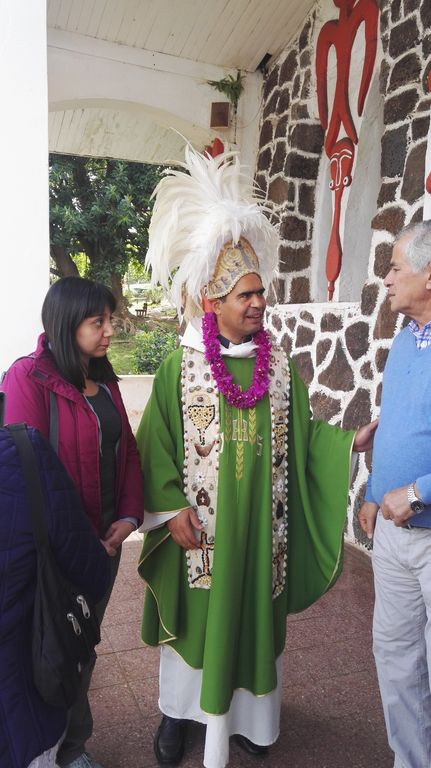
\includegraphics{images/20180827_messe.jpg}
\caption{Le prêtre d'ici et sa coiffe étonnante.}
\end{figure}

Un extrait sonore pour mieux illustrer le propos :

D'ailleurs, connaissez-vous l'origine du mot \emph{Moai} ? D'après Ugo,
notre guide d'un jour, c'est la contraction des mots \emph{mo} et
\emph{ai} qui signifient \emph{pour qui}, ce qui serait lié au fait que
chaque statue de pierre représente un ancêtre donné. Les Moais trônent
(ou plutôt trônaient) donc tout autour de l'île, sur leurs longues
plateformes de pierre, les Ahu, qui servaient aussi de cimetière.

\begin{figure}
\centering
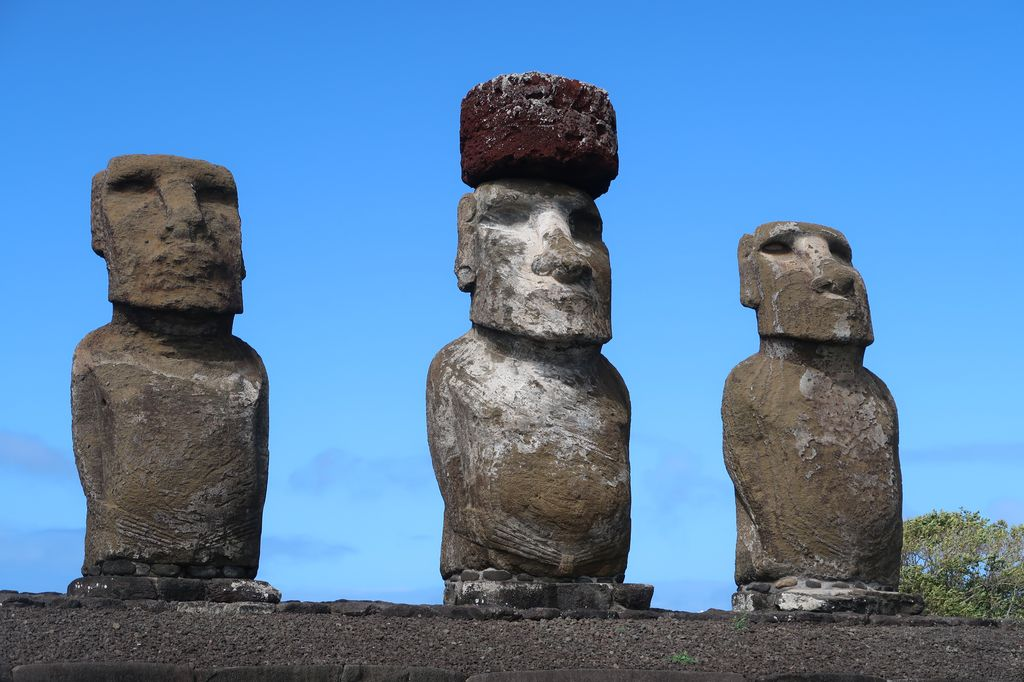
\includegraphics{images/20180827_moai.JPG}
\caption{Plusieurs ancêtres côte à côte. Celui du milieu porte un
chignon de pierre sur sa tête, le \emph{pukao}.}
\end{figure}

La culture Rapa Nui a une histoire mouvementée. Elle aurait été fondée
par des Polynésiens vers le 12ème siècle, et les Ahu avec leurs Moais
seraient une évolution des \emph{marae} comme celui que nous avions vu à
Raiatea, avec une sorte de compétition pour réaliser des Moais de plus
en plus grands. Les plus vieux Moais mesurent 2 mètres, alors que le
plus grand, encore accroché à la montagne dans la carrière de Rano
Raraku, tire plutôt vers les 22 mètres ! Durant la guerre civile, la
totalité des Moais de l'île a été renversée par des clans adversaires,
dans le but d'affaiblir moralement le clan auquel ils appartenaient.
Puis se serait développé avec une chronologie incertaine l'épreuve de
l'homme-oiseau sur le site d'Orongo, qui existait toujours à l'arrivée
des premiers missionnaires continentaux.

\begin{figure}
\centering
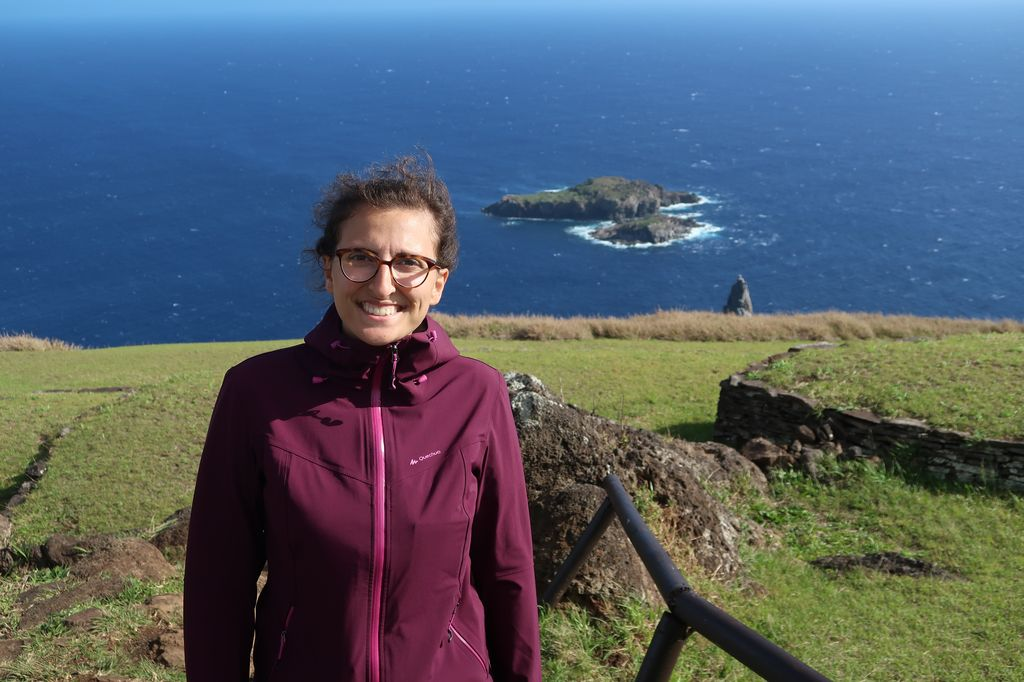
\includegraphics{images/20180827_birdman.JPG}
\caption{Homme-oiseau, mode d'emploi: descendre la falaise en bravant le
vent, nager jusqu'à l'île en évitant les requins, y survivre jusqu'à ce
que l'oiseau ponde, prendre le premier oeuf et revenir, sans le casser.
Facile, non?}
\end{figure}

Après avoir été quasiment détruite suite à la disparition de 97\% de la
population de l'île dans les années 1880, elle s'est reconstruite au fur
et à mesure du temps avec les survivants. Si des tensions avec la
"métropole" chilienne continuent à exister sur l'île (par exemple autour
de l'Eco Lodge, l'un des hôtels), de nombreuses initiatives tentent de
préserver l'héritage Rapa Nui. Comme par exemple le groupe de danse et
d'art Kari Kari, dont nous avons vu le spectacle et dont les artistes
apprennent dès l'enfance à pratiquer tous les arts de leurs ancêtres
(danse, musique, création de costumes, gravure sur bois,...).

\begin{figure}
\centering
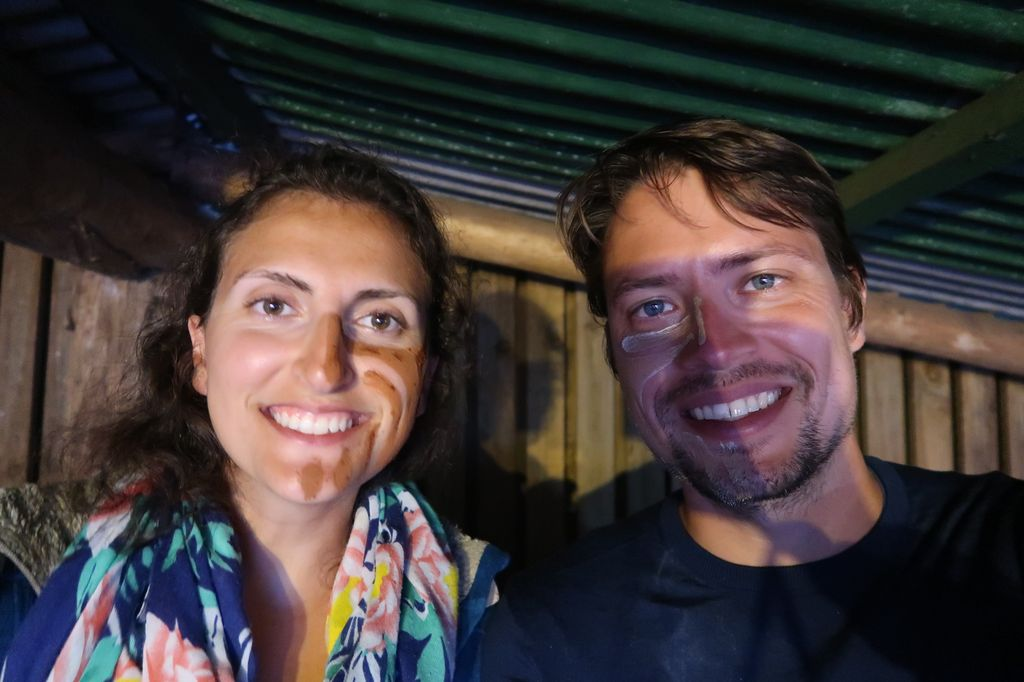
\includegraphics{images/20180827_karikari.JPG}
\caption{Nos visages, à moitié recouverts de peintures traditionnelles à
la terre.}
\end{figure}

Même si une semaine ça peut sembler long pour une île dont on peut faire
le tour à vélo en une journée, c'était tout à fait agréable de découvrir
les mystères de Rapa Nui dans ce laps de temps. On perçoit aussi mieux
l'isolation de l'île au fur et à mesure des changements de météo. Comme
si l'on était sur un bateau perdu dans l'océan Pacifique.

\emph{Florian et Elida}
